\begin{lemma}\label{lem5}
In einem minimalen Gegenbeispiel $\Delta$, kann kein Nachbar $x_i$ einer der Aufhängungen $a_i$ einem Gebiet zugeordnet sein, zu dessen Rand die Kante $(a_i,x_i)$ gehört.
\end{lemma}

\begin{remark}
Lemma \ref{lem5} impliziert insbesondere, dass die drei Aufhängungen $a_1,a_2$ und $a_3$ von $\Delta$ ein Dreieck bilden.
\end{remark}

\begin{proof}
Angenommen es existiert ein Nachbar $x$ von $a_1$, der dem Gebiet $f$ zuwiesen ist und $a_1$ liegt auf dem Rand von $f$. Somit tut dies auch die Kante $(a_1,x)$. Wir werden einen kleineren Graphen $G'$ erstellen und zeigen, dass $G'$ eine SLTR zulässt. Das zu diesem SLTR korrespondierende Schnyder Labeling $\phi'$ kann man dann zu einem Labeling von $G$ erweitern. Im besten Fall kontrahieren wir eine Kante in $G$ um $G'$ zu erhalten ... TODO

Sei $z$ die dritte Ecke des Gebietes $f$ mir den Ecken $a_1$ und $x$. Es kann nur ein solches $z$ geben, da sonst (wie in Abbildung \ref{pic_lem5_1} a) illustriert) ein unterteilendes Dreieck in $\Delta$ existieren müsste. Wir haben aber in Lemma \ref{lem2} gezeigt, dass dies nicht der Fall sein kann.

Wir können davon ausgehen, dass $z$ und $a_1$ benachbart sind. Falls nicht muss ein Knoten $x'$ zwischen $z$ und $a_1$ liegen. Sei $z'$ die Dritte Ecke im Gebiet mit Ecken $a_1,x',z'$. $x'$ muss in diesem Gebiet eine Ecke sein, da es im zuerst betrachteten zugewiesen ist (siehe Abbildung \ref{pic_lem5_1}, b)). Nun ist entweder $z'$ ein Nachbar von $a_1$, oder wir führen den Schritt noch einmal durch und finden $x''$. Da $a_1$ endlich viele Nachbarn hat können wir den Schritt und endlich oft durchführen. Es existiert also ein Gebiet mit $a_1, x$ und $z$ als Ecken und $x$ und $z$ sind Nachbarn von $a_1$. Es sei angemerkt, dass $x$ am äusseren Gebiet von $G$ liegen kann.

\begin{figure}
	\centering
	  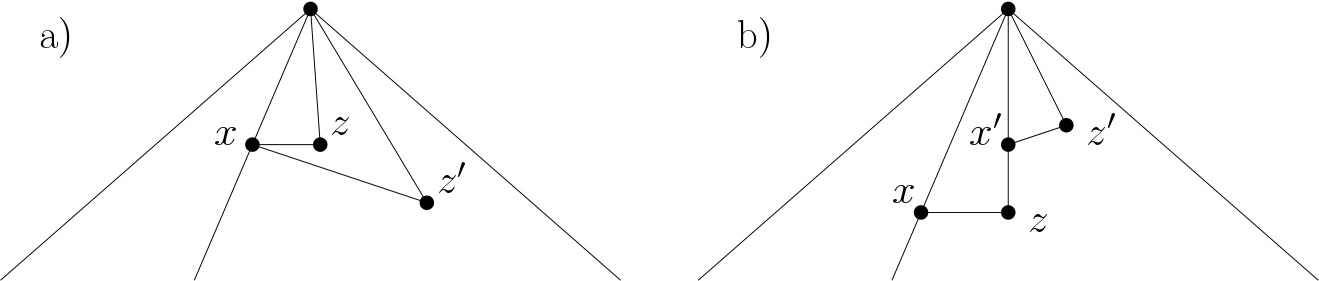
\includegraphics[width=0.8\textwidth]{lem5_1.png}
    	\caption{a) Es können keine zwei Knoten mit geradlinigen Pfaden zu $x$ und $a_1$ existieren. b) Falls $a_1$ kein Nachbar von $z$ ist, dann müssen die Knoten $x'$ und $z'$ existieren.}
    	\label{pic_lem5_1}
\end{figure}

Wir werden je nach Fall unterschiedliche Ansätze wählen, um $G'$ zu erzeugen. Es folgt eine Übersicht der Fälle, die in Abbildung \ref{pic_lem5_2} skizziert sind.

\begin{itemize}
\item [1.] $x$ und $z$ sind Nachbarn.
	\begin{itemize}
	\item [a)] Falls $z$ dem Gebiet auf der anderen Seite von $(x,z)$ zugewiesen ist, dann kontrahieren wir $(x,z)$.
	\item [b)] Falls $deg(z)$=3 gilt, löschen wir $z$ und fügen eine passende Kante ein.
	\item [c)] Falls $(a_1,x)$ kontrahierbar ist wird sie kontrahiert.
	\item [d)] Sonst wird die Kante $(a_1,z)$ gelöscht.
	\end{itemize}
\item [2.] $x$ und $z$ sind keine Nachbarn, dann kontrahieren wir die Kante $(a_1,x)$.
\end{itemize} 

\begin{figure}
	\centering
	  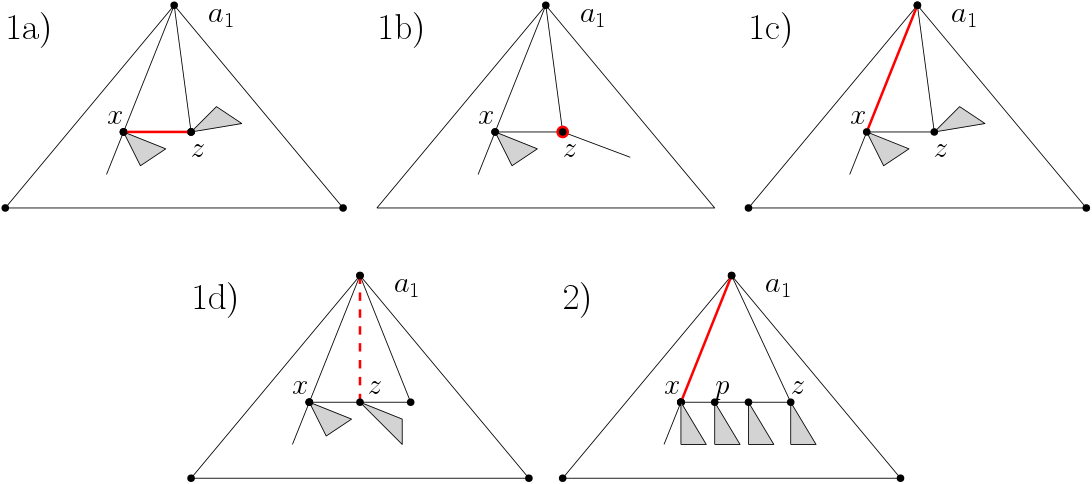
\includegraphics[width=0.8\textwidth]{lem5_2.png}
    	\caption{Die möglichen Fälle bei der Erzeugung von $G'$. Die durchgezogenen roten Kanten werden kontrahiert. Der rote Knoten und die gestrichelte rote Kante gelöscht.}
    	\label{pic_lem5_2}
\end{figure}

Für jeden dieser Fälle entsteht ein ein Graph $G'$ der kleiner ist als $G$ und eine SLTR zulässt. Da er kein Gegenbeispiel sein kann besitzt er ein Ecken kompatibles Paar. Das involvierte Schnyder Labeling lässt sich zu einem für $G$ erweitern und dieses ist Ecken kompatibel mit dem von $\Delta$ induzierten FAA. Wir werden uns jetzt den einzelnen Fällen im Genaueren zuwenden. 

\underline{Fall 1a}: $(x,z)$ ist eine Kante und somit $s,z,a_1$ ein echtes Dreieck. Um $G'$ zu erzeugen, löschen wir $(a_1,z)$ und kontrahieren $(x,z)$. Wir bezeichnen den neuen Knoten mit $x'$ (siehe Abbildung \ref{pic_lem5_3}). Wir erhalten dass FAA $\phi'$ indem wir die Zuweisung von $x$ aus $\phi$ löschen.





\end{proof}